\documentclass[border=1]{standalone}
\usepackage{tikz}
\usepackage{xcolor}
\tikzset{
    point/.style={ fill }
}

\begin{document}
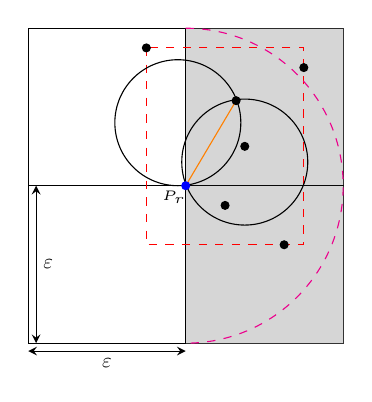
\begin{tikzpicture}
\coordinate (O) at (0,0);
\coordinate (A) at (0,2);
\coordinate (B) at (4,0);
\coordinate (C) at (0,4);
\coordinate (D) at (2,0);
\coordinate (E) at (2,2);
\coordinate (F) at (2,4);
\coordinate (G) at (4,4);
\coordinate (H) at (4,2);

\draw[] (O) -- (A) -- (E) -- (D) -- cycle;
\draw[] (A) -- (E) -- (F) -- (C) -- cycle;
\draw[fill=black!20,opacity=0.8] (E) -- (H) -- (G) -- (F) -- cycle;
\draw[fill=black!20,opacity=0.8] (D) -- (B) -- (H) -- (E) -- cycle;

\draw[stealth-stealth] (0.1, 0) -- node[scale=0.75, right]{$\varepsilon$}(0.1, 2);
\draw[stealth-stealth] (0, -0.1) -- node[scale=0.75, below] {$\varepsilon$}(2, -0.1);


\coordinate (B0) at (1.50, 3.75);
\coordinate (B1) at (1.50, 1.25);
\coordinate (B2) at (3.50, 1.25);
\coordinate (B3) at (3.50, 3.75);
\draw[dashed, red] (B0) -- (B1) -- (B2) -- (B3) -- cycle;

\coordinate (C1) at (1.90, 2.80); \draw[] (C1) circle (0.8);
\coordinate (C2) at (2.75, 2.30); \draw[] (C2) circle (0.8);

\coordinate (P0) at (2.00, 2.00); 
\draw[magenta, dashed] (2.00, 4.00) arc (90:-90:2.00);

\coordinate (P1) at (2.50, 1.75); \draw[point] (P1) circle (0.05);
\coordinate (P2) at (2.75, 2.50); \draw[point] (P2) circle (0.05);
\coordinate (P3) at (3.25, 1.25); \draw[point] (P3) circle (0.05);
%\coordinate (P4) at (2.50, 3.00); \draw[point] (P4) circle (0.05);
\coordinate (P5) at (3.50, 3.50); \draw[point] (P5) circle (0.05);
\coordinate (P6) at (1.50, 3.75); \draw[point] (P6) circle (0.05);
\coordinate (P7) at (2.64, 3.08); 
\draw[orange] (P0) -- (P7);
\draw[point] (P7) circle (0.05);

\draw[point, color=blue] (P0) circle (0.05);
\node[] at (1.85,1.85) {\tiny $P_r$};

\end{tikzpicture}
\end{document}
